\begin{figure}[h]
  \begin{subfigure}{\linewidth}
    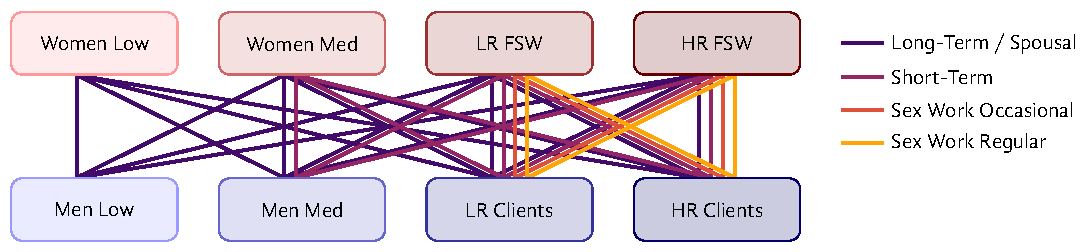
\includegraphics[scale=.8]{model.risk}
    \caption{Activity groups and partnership types}
    \label{fig:model.risk\mfx}
  \end{subfigure}
  \begin{subfigure}{\linewidth}
    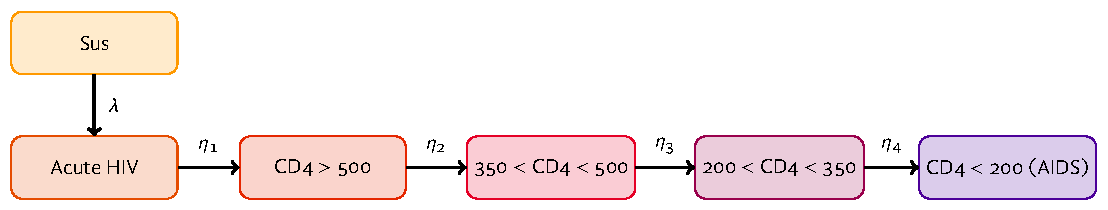
\includegraphics[scale=.8]{model.hiv}
    \caption{HIV states}
    \label{fig:model.hiv\mfx}
  \end{subfigure}
  \begin{subfigure}{\linewidth}
    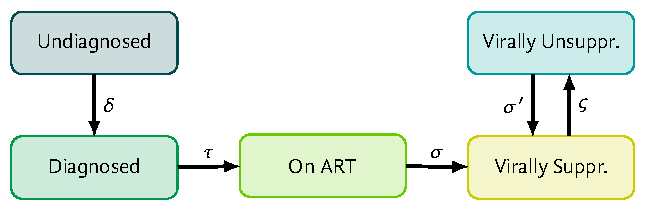
\includegraphics[scale=.8]{model.cascade}
    \caption{ART cascade states}
    \label{fig:model.cascade\mfx}
  \end{subfigure}
  \caption{Model structure and transitions}
  \label{fig:model\mfx}
  \floatfoot{
    \ffpops;
    CD4: CD4+ T-cell count per mm\tsup{3};
    ART: antiretroviral therapy;
    rates ---
    $\lambda$: force of infection;
    $\eta$: HIV progression;
    $\delta$: diagnosis;
    $\tau$: ART initiation;
    $\sigma$: viral suppression;
    $\sigma'$: viral re-suppression;
    $\varsigma$: ART failure / discontinuation;
    not shown: turnover amongst activity groups in \sfref{fig:model.risk}.}
\end{figure}
